\section{Generierung von Vorschlägen für Variablen-Belegungen}\label{chap:testdatasuggestions}

Um dem Entwickler repräsentative Testwerte, die die Variationspunkte eines SQL-Statements beeinflussen, vorzuschlagen, gibt es verschiedene Strategien.
Grundlage dafür bietet neben dem Quelltext, ein Datenbanksystem mit den enthaltenen Echt-Daten.
In den folgenden Beispielen werden Unternehmensdaten aus einer SAP-Infrastruktur einer Aktiengesellschaft genutzt.
Die Integration solcher Datenbanksysteme und die Administration von den genutzten Test-Daten werden im Kapitel \ref{chap:testdataadministration} ausführlicher behandelt.

Neben der Betrachtung der Charakteristiken von Daten innerhalb der Datenbank und dem Kontext aus dem Quelltext, ist vor allem die Verknüpfung mit Analyse-Ergebnissen, vorrangig den Laufzeit-Messungen, ein Kriterium für die Generierung der Vorschläge.
Mittels Auswahl unterschiedlicher, vorgeschlagener Testwerte ist es dem Entwickler möglich konkrete Ausprägungen von SQL-Statements nachzuvollziehen und durch die Auswertung der Messungen gegebenenfalls Optimierungen durchzuführen bis das gewünschte Performance-Verhalten erreicht ist.
Doch zuerst müssen die Variablen ermittelt werden, die einen Einfluss auf das SQL-Statement haben.

\subsection{Bestimmung der zu betrachtenden Variablen}
Kapitel \ref{sec:controlflowandsqldependencies} zeigte bereits auf, dass Variablen in unterschiedlichen Weisen auf ein SQL-Statement einwirken können.
Dies schlägt sich auch auf die Vorschlagsgenerierung nieder.
Um die Variablen, die auf ein SQL-Statement Einfluss nehmen, zu bestimmen, dient die Schnittstelle \texttt{javascriptParser.getSqlQueryAtPosition()} des Quelltext-Parsers von \cite{Horschig2014}.
Sie liefert ein Objekt zurück mit zwei wichtigen Attributen: \texttt{dependencies} und \texttt{variables}.
Dabei enthält \texttt{dependencies} alle Variablen, von den das SQL-Statement im Kontrollfluss abhängig ist, wohingegen \texttt{variables} alle Variablen umfasst, die innerhalb des SQL-Statements auftreten.
Darüber hinaus können Variablen auch in beiden Listen vorkommen.
Die Zuordnung erfolgt in diesem Fall anhand des Attributs \texttt{uniqueName}.
Die Elemente in \texttt{variables} enthalten zusätzlich Kontext-Informationen, die eine Zuordnung zu Spalten innerhalb einer Relation ermöglichen, und so die Grundlage für die Generierung von Testdaten-Vorschläge schaffen.
In Abbildung \ref{fig:querytree} ist eine solche Datenstruktur beispielhaft für das Code-Beispiel \ref{lst:differentdep} dargestellt.

\begin{figure}[ht]
	\centering
	\scalebox{.58}{
		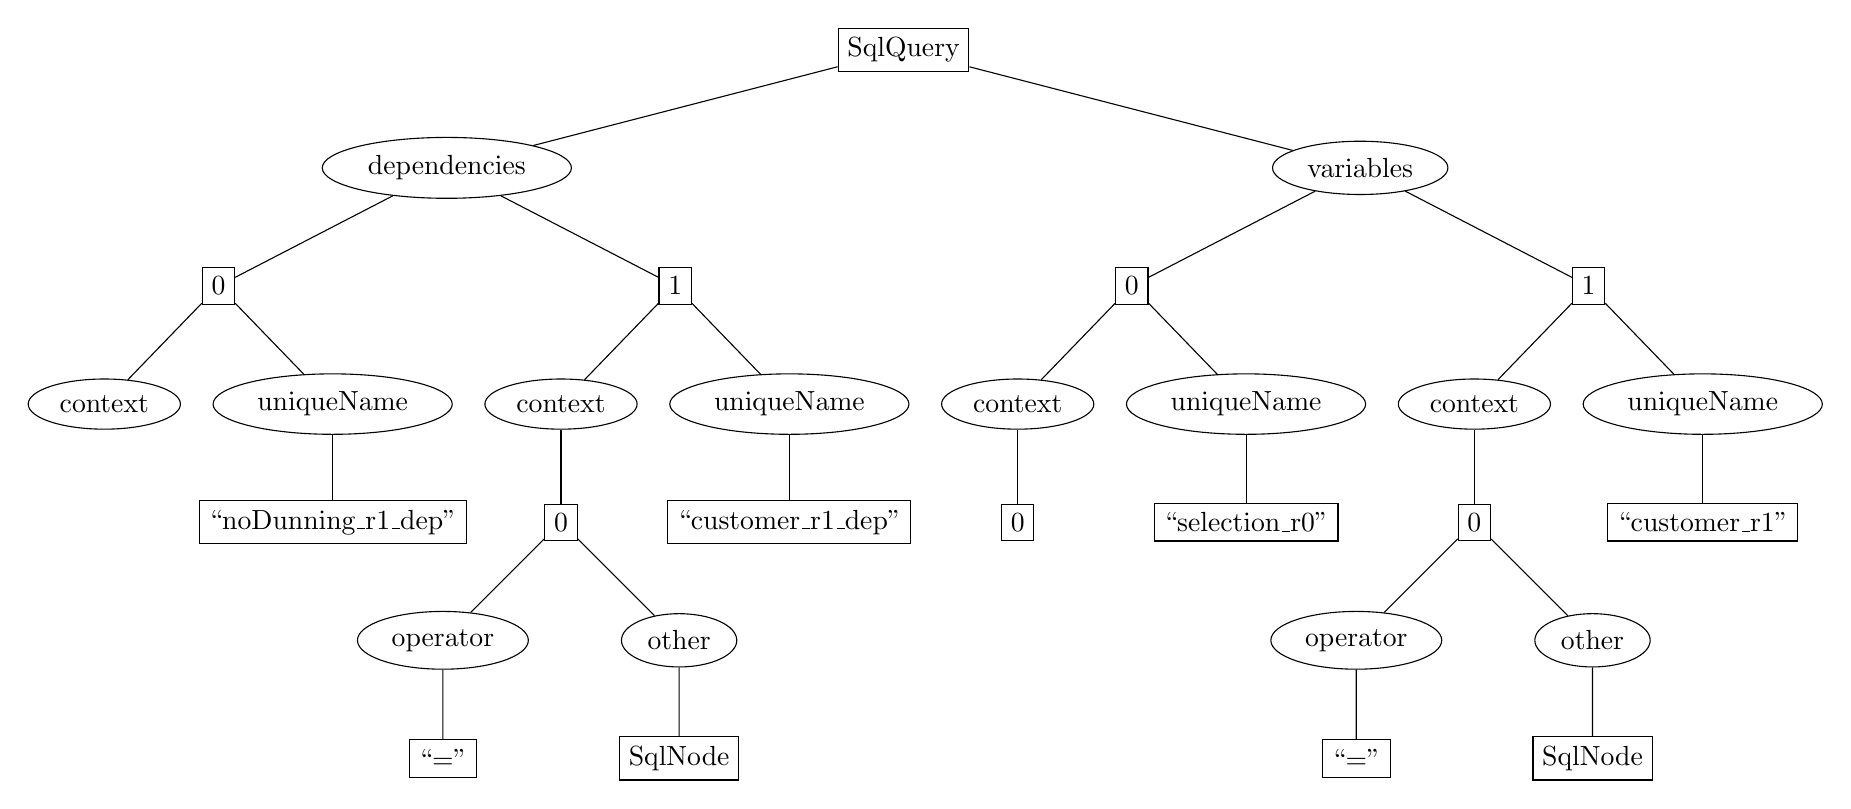
\begin{tikzpicture}
			\usetikzlibrary{shapes}
			\tikzstyle{e} = [draw, shape=ellipse]
			\tikzstyle{r} = [draw, shape=rectangle]
			\node[r] (is-root) {SqlQuery}
				[sibling distance=11.6cm]
				child { 
					node[e] {dependencies}
					[sibling distance=5.8cm]
					child {
						node[r] {0}
						[sibling distance=2.9cm]
						child { node[e] {context} }
						child {
							node[e] {uniqueName}
							child { node[r] {``noDunning\_r1\_dep''} }
						}
					}
					child {
						node[r] {1}
						[sibling distance=2.9cm]
						child { 
							node[e] {context} 
							child {
								node[r] {0}
								[sibling distance=3cm]
								child {
									node[e] {operator} 
									child { node[r] {``=''} }
								}
								child {
									node[e] {other} 
									child { node[r] {SqlNode} }
								}
							}
						}
						child {
							node[e] {uniqueName}
							child { node[r] {``customer\_r1\_dep''} }
						}
					}
				}
				child { 
					node[e] {variables}
					[sibling distance=5.8cm]
					child {
						node[r] {0}
						[sibling distance=2.9cm]
						child { 
							node[e] {context} 
							child { node[r] {0} }
						}
						child {
							node[e] {uniqueName}
							child { node[r] {``selection\_r0''} }
						}
					}
					child {
						node[r] {1}
						[sibling distance=2.9cm]
						child { 
							node[e] {context} 
							child {
								node[r] {0}
								[sibling distance=3cm]
								child {
									node[e] {operator} 
									child { node[r] {``=''} }
								}
								child {
									node[e] {other} 
									child { node[r] {SqlNode} }
								}
							}
						}
						child {
							node[e] {uniqueName}
							child { node[r] {``customer\_r1''} }
						}
					}
				};
		\end{tikzpicture}
	}
	
	

	\caption{Verteilung distinkter Werten einer Auswahl von Spalten aus BSEG}
	\label{fig:querytree}
\end{figure}


\subsection{Vorschläge auf Basis von Daten-Charakteristiken}\label{chap:datacharacteristics}
Sobald Variablen nicht nur die Gestalt eines SQL-Statements variieren, sondern auch darin einfließen, ist der erste Anhaltspunkt für das Vorschlagen relevanter Testwerte die Charakteristik der Datenbankinhalte.
Für Selektionsfilter spielt dabei primär die Verteilung der Daten innerhalb der Relationen eine Rolle, sowie die Anzahl ihrer unterschiedlichen Werte-Ausprägungen.
Im Gegensatz dazu werden für Projektion, Sortierung und Gruppierung Meta-Informationen zu den Relationen der Datenbank berücksichtigt.
Zweiteres wird im Kapitel \ref{chap:databasemeta} näher betrachtet.

%\begin{figure}
%\centering
	%\begin{tikzpicture}
		%\begin{axis}[
				%axis lines=left,
				%width  = 0.85*\textwidth,
				%height  = 6cm,
				%symbolic x coords={Males,Females},
				%xtick=data,
				%enlarge x limits=0.5,
				%bar width=40pt,
				%ybar,
				%ylabel={Percentage},
				%ymin=0.0,
				%ymax=100.0,
				%]
				%\addplot[ybar,fill=light-gray] coordinates {
						%(Males,55)
						%(Females,45)
				%};
		%\end{axis}
	%\end{tikzpicture}
	%\caption{(TODO: ersetzten durch statistik in BSEG.) Verteilung der Werte in der Spalte Gender.}
	%\label{fig:gender}
%\end{figure}

\pgfkeys{
    /pgf/number format/precision=0,
    /pgf/number format/fixed zerofill=true,
    /pgf/number format/fixed,
		/pgf/number format/.cd,
		use comma,
		1000 sep={.}
}

\begin{figure}[ht]
\centering
	\begin{tikzpicture}
		\begin{axis}[
			axis lines=left,
			xbar, xmin=0,
			width=0.85*\textwidth,
			height=6cm,
			enlarge y limits=0.1,
			xlabel={Absolute Anzahl distinkter Werte},
			symbolic y coords={MANDT,GJAHR,ZLSCH,BUKRS,AUGDT,LIFNR,SKFBT,KUNNR,WRBTR,BELNR},
			ytick=data,
			bar width=5pt,
			nodes near coords, nodes near coords align={horizontal},
			]
			\addplot[fill=light-gray] coordinates {
				(5636590,BELNR)
				(560628,WRBTR)
				(408015,KUNNR)
				(228722,SKFBT)
				(48407,LIFNR)
				(2304,AUGDT)
				(71,BUKRS)
				(31,ZLSCH)
				(10,GJAHR)
				(2,MANDT)
			};
		\end{axis}
	\end{tikzpicture}
	\caption{Verteilung distinkter Werten einer Auswahl von Spalten aus BSEG}
	\label{fig:bseg}
\end{figure}

Die Abbildung \ref{fig:bseg} zeigt eine Auswahl der 326 Spalten der BSEG-Tabelle aus einem SAP-System.
Die Tabelle enthält alle einzelnen Belegpositionen zu den Buchungsbelegen des Unternehmens.
Eine Erläuterung zu der Bedeutung der einzelnen Spalten befindet sich im Anhang (Tabelle \ref{tab:bsegerlaeuterung}).

Sollte die Anzahl der distinkten Werte einstellig sein (beispielsweise bei der Spalte MANDT), können dem Entwickler alle möglichen Ausprägungen in einem Auswahl-Menü zur Verfügung gestellt werden.
Damit wird gleichzeitig auch sichergestellt, dass nur Werte eingegeben werden können, die beim testweisen Ausführen des SQL-Statements ein Ergebnis zurückgeben.
Auf der anderen Seite können sich Spalten jedoch über eine große Menge von verschiedenen Datenausprägungen erstrecken, wie zum Beispiel bei Belegnummern (BELNR), was eine einfache Auswahl passender Testdaten kompliziert gestaltet.
Für diesen Fall werden Äquivalenzklassen anhand der Vorkommen der Werte erzeugt, die sich unterteilen in: die drei häufigsten Werte, die drei seltensten Werte, drei Werte um den Median und der Rest.

Für die häufigsten Werte wird eine aufsteigende Sortierung der Anzahl des Vorkommens eines Wertes vorgenommen und die ersten drei selektiert.
Sollten mehrere Werte dieselbe Anzahl an Vorkommen vorweisen, werden sie zusätzlich anhand ihrer Werte aufsteigend sortiert.
Im Unterschied dazu wird bei der Klasse der seltensten Werten initiale ein absteigende Sortierung vorgenommen.
Für die Werte um den Median muss zuerst die Anzahl der verschiedene Werte ermittelt werden.
Anschließend dient die Halbierung des Ergebnisses als Offset für die Bestimmung der drei vorzuschlagenden Werte.
Die SQL-Statements dazu befinden sich im Anhang als Code-Beispiel \ref{lst:distinctvalues}.

\subsection{Vorschläge anhand von Meta-Informationen}\label{chap:databasemeta}
Für Projektion, Sortierung oder Gruppierung sind weniger die Spalte-Inhalte wichtig, als vielmehr die Spalten an sich.
Um Vorschläge für diese Art SQL-Statement-Variablen zu erzeugen, werden dazu anhand der Meta-Informationen über Spalten der betrachteten Relation aus der SAP Hana-internen System-Tabelle \texttt{SYS.TABLE\_COLUMNS} die Spalten-Namen bestimmt (vgl. Code-Beispiel\ref{lst:hanasys}).
\begin{lstlisting}[caption={Systemtabellen von SAP Hana liefern Meta-Informationen zu Relationen}, label={lst:hanasys}, language=SQL]
	SELECT COLUMN_NAME
	FROM SYS.TABLE_COLUMNS
	WHERE SCHEMA_NAME = '<schema>'
	AND TABLE_NAME = '<table>'
\end{lstlisting}
Die notwendigen Informationen (Schema und Tabelle) werden dazu dem SQL-Statement entnommen.

\subsubsection{Nutzung von Meta-Informationen für UI-Elemente}
Die Meta-Informationen zu Spalten umfassen neben den Namen auch noch weitere nützliche Informationen, die die Eingabe von Testdaten unterstützen können.
Beispielsweise können der Datentyp von Spalten (\texttt{DATA\_TYPE\_NAME}), die Erlaubnis der Eingabe von NULL-Werten (\texttt{IS\_NULLABLE}) oder auch die Länge (\texttt{LENGTH}) für die Erstellung der Eingabefelder genutzt werden kann.
So kann die Eingabe, die eine Spalte mit Datumsangaben referenziert, durch einen Kalender vereinfacht werden.
Auch die Einschränkung auf Datentypen, z.B. Ganzzahlen, kann fehlerhafte Eingabe durch den Entwickler verhindern.
Eine weitere Unterstützung ist die Autovervollständigung von teilweise eingegeben Werten.
Mittels des SQL-Operators \texttt{LIKE} kann dazu nach Daten gesucht werden, die dem Muster der bisherigen Eingabe entsprechen.
Diese Zusatzinformationen erhöhen die Komfortabilität der Eingabe und können fehlerhafte Eingaben reduzieren.

\subsection{Adaptive Vorschlagsgenerierung durch Laufzeit-Analysen}\label{chap:adaptive}
Der in Kapitel \ref{chap:datacharacteristics} vorgestelle Ansatz zum Vorschlage einzelner Testwerte stößt an seine Grenzen, sobald mehrere Parameter genutzt werden und diese voneinander abhängig sind.
Im Code-Beispiel \ref{lst:dynamicsql} aus dem Kapitel \ref{sec:dependencydetection} werden beispielsweise offene Rechnungen und deren Einzelposten gesucht.
Die Variable \texttt{customer} gibt dabei die Kundennummer an, mit der die Rechnungen assoziiert sind.
Sucht man nun nach der Kundennummer mit den meisten Rechnungen, bedeutet dies nicht zwangsläufig, dass man auch die mit den meisten Einzelposten oder höchsten Gesamtsummen findet.
Diese, noch recht einfache, Abhängigkeit kann beliebig erweitert werden.
Damit entstehen komplexe SQL- und Programm-Strukturen, die durch das einfache Vorschlagen anhand von Charakteristiken einzelner Spalten nicht zwangsläufig die Randfälle aufzeigen, die der Entwickler sucht.
Aus diesem Grund ist die Betrachtung von Messegebnissen aus Laufzeit-Analysen (\cite{Exner2014}, \cite{Mues2014}) eine sinnvolle Erweiterung um die Genauigkeit der Vorschläge zu steigern.
Die variablen Stellen von SQL-Statements werden dabei durch die vom Entwickler ausgewählten Werte gefüllt.
Im nächsten Schritt werden nun diese atomaren Vorschläge kombiniert und mit dem dazugehörigen Ergebnis aus der Laufzeit-Analyse verknüpft.
Dies ermöglicht Vergleichbarkeit verschiedener Konstellationen.
Für die Erstellung der initialen Daten können zwei verschiedene Ansätze verfolgt werden.

Mithilfe der Brute-Force-Methode können alle Kombinationen durchprobiert und gemessen werden.
Der enorme Aufwand, gerade bei besonders Relationen mit vielen Einträgen und distinkten Werten in den Spalten, stellt jedoch aufgrund der enormen Berechnungszeit ein großes Hindernis dar.

Dem gegenüber steht der adaptive Ansatz, bei dem der Testdaten-Bestand kontinuierlich erweitert wird.
Diese Variante speichert die Ergebnisse der Laufzeit-Analysen mit den dazugehören Testdaten-Konstellationen als Testdaten-Sets.
Sobald mehrere dieser Sets vorhanden sind, können dem Entwickler drei Vorauswahl-Optionen gegeben: das Testdaten-Set mit der höchsten Laufzeit, mit der geringsten Laufzeit und mittlerer Laufzeit.

Um für diese Methode eine Datengrundlage zu schaffen, werden die in Kapitel \ref{chap:datacharacteristics} ermittelten Werte genutzt um initiale Kombinationen zu bilden und ihre Laufzeiten zu berechnen.
Durch Eingabe weiterer Werte durch den Entwickler kann anschließend das Datenmodell kontinuierlich erweitert und zunehmend verbessert werden, zu sehen im Code-Beispiel \ref{lst:developerinput}.

\begin{lstlisting}[caption={Eingaben von Testwert-Konstellationen erweitern gegebenenfalls das Datenmodell}, label={lst:developerinput}, language=Python]
	hier
	kommt
	der
	algorithmus
	rein
\end{lstlisting}

TODO: Algorithmus beschreiben.

\subsection{Betrachtung von Zeitbereichsanfragen}
Ein typischer Bestandteil von Datenbankanfragen in Geschäftsanwendungen sind Bereichsfilter mittels \texttt{column BETWEEN x AND y},  insbesondere für Zeiträume.
Der in Kapitel \ref{chap:datacharacteristics} vorgestellte Algorithmus generiert Vorschläge basierend auf binären Operationen (zumeist Vergleiche), wohingegen ein Bereichsfilter ternär ist.
Deshalb ist eine besondere Betrachtung für passende Vorschläge sinnvoll.

Sollte eine Bereichsanfrage erkannt werden, die eine Spalte vom Datentyp \texttt{DATE} referenziert, so kann der Entwickler eine vorgeschlagene Zeitraumgröße (z.B. eine Woche, ein Monat oder ein Jahr) auswählen oder selbst festlegen.
Anschließend wird die referenzierte Spalte mithilfe der angegebenen Zeitraumgröße gescannt, ähnlich dem Prinzip des Sliding Window\footnote{\url{http://en.wikipedia.org/wiki/Sliding_window_protocol}}.
Auf dieser Basis werden, ähnlich dem Algorithmus aus Kapitel \ref{chap:datacharacteristics}, bis zu 3 Vorschläge für die größte, kleinste und mittlere Anzahl an Resultaten erzeugt.
Alternativ steht es dem Entwickler offen, Start- und Enddatum eigenständig festzulegen.

\subsection{Vorschläge für Variablenwerte ohne Datenbankbezug}

TODO

\subsection{Integration in die IDE}
\begin{figure}[ht]
	\centering
  \includegraphics[width=0.4\textwidth]{figures/integration.png}
	\caption{Einbindung der Vorschläge in die Sidebar der Web-IDE}
	\label{fig:ideintegration}
\end{figure}

Die in Kapitel \ref{chap:datacharacteristics} und \ref{chap:adaptive} erzeugten Vorschläge werden in der zur Web-IDE gehörenden Datenbank gespeichert und in einer Sidebar im Frontend eingebunden (vgl. Abbildung \ref{fig:ideintegration}).
Durch das Auswählen des Entwicklers einer Quelltext-Zeile mit SQL-Inhalt, werden die Informationen zu dem dazugehörigen SQL-Statement aggregiert und aufbereitet (vgl. Kapitel \ref{chap:entwicklungsumgebung}) und schließlich in der Sidebar angezeigt.

Aus der im Kapitel \ref{chap:adaptive} ermittelten Menge an Testdaten-Sets werden zum einen die drei mit der höchsten, geringsten und durchschnittlichen Laufzeit angeboten, zum anderen ein Auswahl-Menü mit allen gespeicherten Sets.
Die Auswahl einer dieser Optionen füllt die Eingabefelder für die Testdaten automatisch mit den gespeicherten Werten und löst eine Analyse aus.
Möchte der Entwickler weitere Testdaten-Sets hinzufügen, so kann er diese benennen und direkt abspeichern.
Die Verwaltung dieser gespeicherten Daten wird im folgenden Kapitel behandelt.